\chapter{Revisão Bibliográfica}

A grande maioria dos medicamentos, neutralizam a IL-6R mediante a interferência na ligação IL-6/gp80, afetando tanto a sinalização clássica quanto a trans-sinalização da IL-6. A proteína sgp130Fc, também denominada de sIL-6R subunidade $\beta$, bloqueia especificamente a trans-sinalização de IL-6 sem afetar a sinalização clássica. \cite{Simon2011} A forma solúvel de IL-6R (sIL-6R), que compreende o domínio extracelular do receptor, está envolvida em diversos processos pró-inflamatórios no organismo. \cite{Stefan2012} 

\section{Estrutura cristalográfica da interleucina sIL-6R subunidade $\alpha$}

Mediante a base de dados, Protein Data Bank(PDB), foram encontradas 8 estruturas proteicas expressas pelo ser humano(\textit{Homo sapiens}) que correspondem à palavra-chave: IL-6R. Os dois métodos de caracterização encontrados correspondem a NMR e XRD. No entanto, muitas estruturas estão incompletas por possíveis falhas na cristalização. Até o momento, existem apenas 2 estruturas com quantidade de resíduos superior a ($90\%$) pertencentes a uma região favorável no diagrama de Ramanchandran.

Para que haja a convicção de que o receptor é de fato a forma solúvel da proteína IL-R$\alpha$, foi realizada uma busca no catálogo da fabricante $Sigma-Aldrich$, onde a proteína recombinante sIL-R$\alpha$ possui o código $SRP3097$. Desta forma, por intermédio da ferramenta $Phyre2$ foi inserido a sequência de alinhamento de aminoácidos fornecido pela $Sigma-Aldrich$ no intuito de encontrar uma proteína homóloga, e portanto, a que será utilizada nesta pesquisa.     

\begin{figure}[H]
\centering
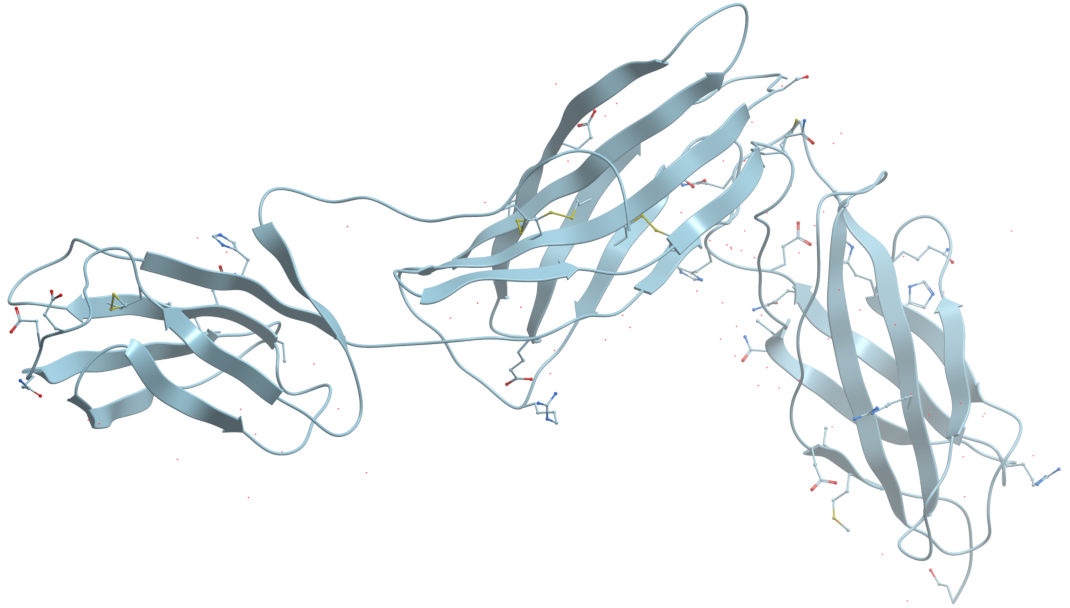
\includegraphics[scale=1.2]{Figuras/il6-ra.png}
\caption{Visualização estrutural por meio do software \textit{ICM-Browser} dos domínios extracelulares da proteína IL-6R(PDB ID: 1N26, cadeia $\alpha$), também denominado de sIL-6R. \cite{Varghese2002}}
\end{figure}

A proteína foi validada pela ferramenta RAMPAGE (Ramachandran Plot Investigation). Após a submissão do arquivo \texiit{.pdb}, a estrutura demonstrou que $90,6\%$ dos resíduos estavam presentes em uma região favorecida, embora outros $6,4\%$ dos resíduos compreenderam a área limite, e $3,0\%$ em condições de exceção. Mediante esses parâmetros, percebe-se uma excelente qualidade estrutural.

\begin{figure}[H]
\centering
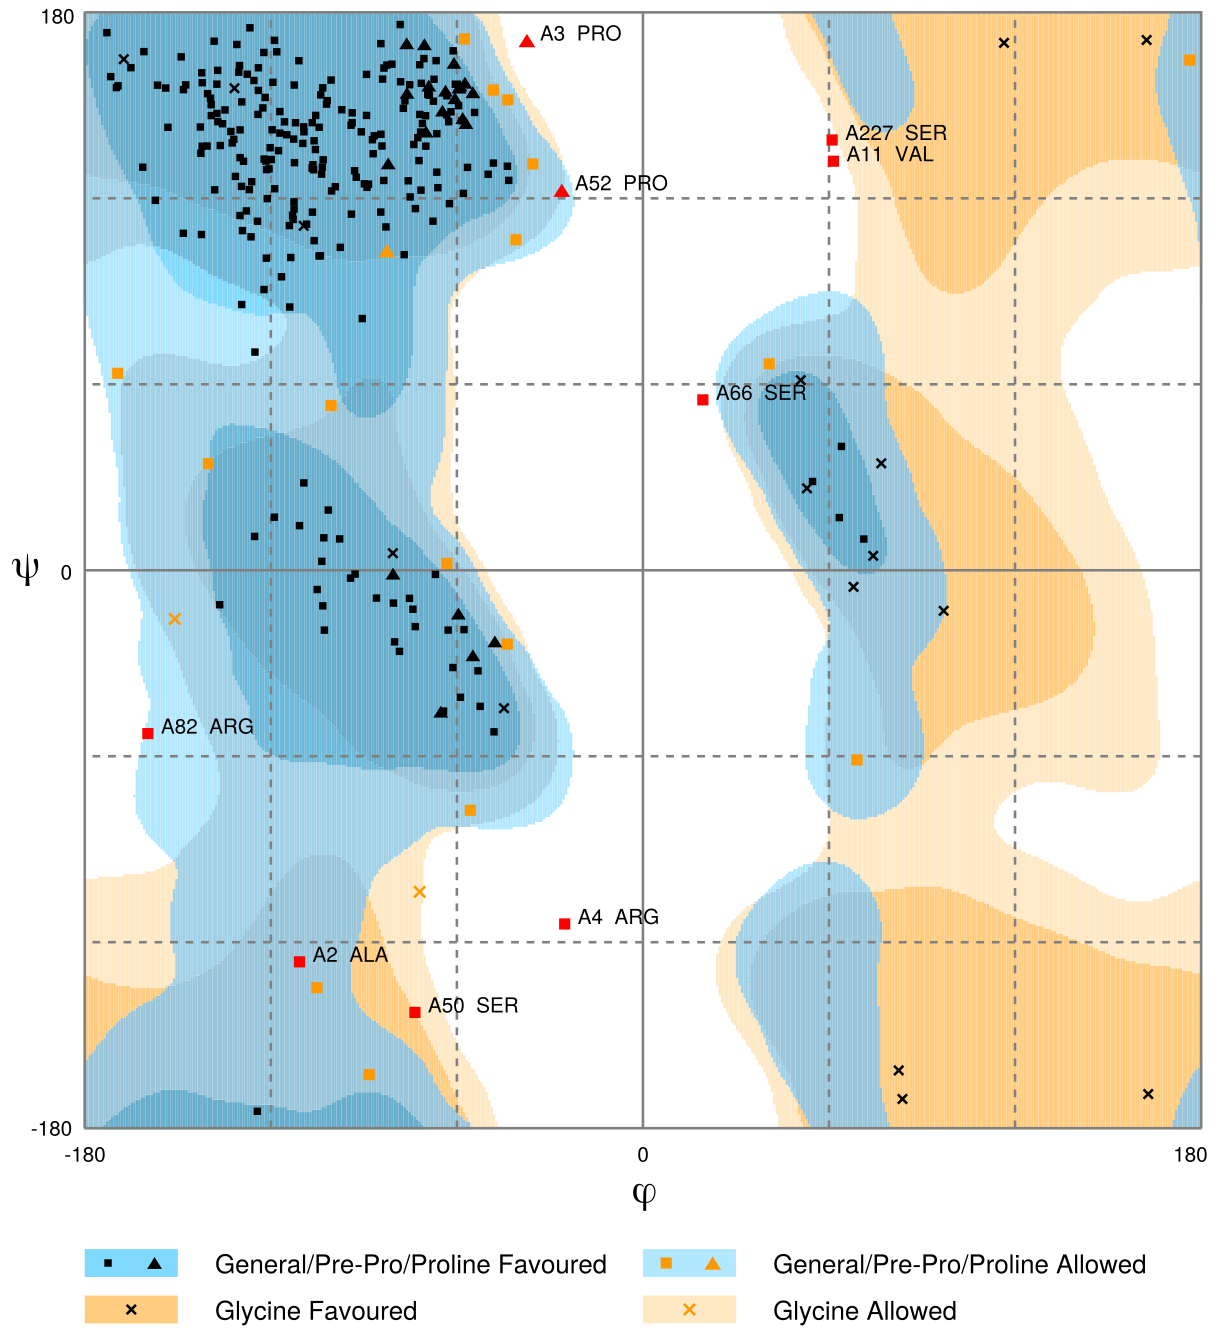
\includegraphics[scale=0.6]{Figuras/ramachandran_1n26.png}
\caption{Análise estrutural da proteína sIL-6R mediante o mapa de Ramanchandran calculado por intermédio da ferramenta RAMPAGE. \cite{Ramanchandran2003}}
\end{figure}

\section{Sinalização clássica e trans-sinalização da interleucina-6}

A interleucina-6 é uma citocina não apenas envolvida nas respostas à inflamação e infecção, mas também na regulação de processos metabólicos, regenerativos e neurais. Em vários modelos, foi demonstrado que a sinalização clássica de IL-6 tem a função de mediar a ativação de vias anti-inflamatórias nas células-alvo. Em contraste, a trans-sinalização de IL-6 é observada em pacientes com doenças inflamatórias crônicas. \cite{Scheller2011}

A IL-6 tem uma ação dicotômica no CNC, exibindo propriedades neurotróficas, por um lado, e ações prejudiciais, por outro. Isso está de acordo com seu papel central na
neuroinflamação, que evoluiu como um processo benéfico, destinado a manter os tecidos em homeostase, mas que pode se tornar maligna quando em excesso. \cite{Spooren2011} Nesta perspectiva, é importante compreender os corretos mecanismos de inibição que possam trazer recuperação, ao invés de danos à saúde. A IL-6 é considerado uma proteína promissora para a intervenção clínica. Contudo, a sinalização que controla sua atividade é complexa, e distintas estratégias de intervenção podem inibir essa via. \cite{Jones2015}


\begin{figure}[H]
\centering
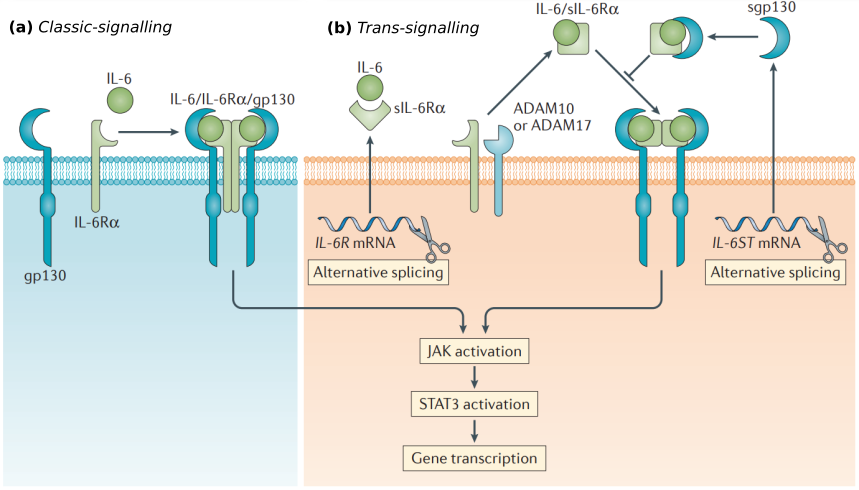
\includegraphics[scale=1]{Figuras/signalling_il6.png}
\caption{Vias de sinalização da interleucina-6. (a) Na sinalização clássica, emerge uma atividade anti-inflamatória. (b) Na trans-sinalização, emerge uma atividade pro-inflamatória. \cite{Johnson2018} (Adaptado)}
\end{figure}

\section{Triagem virtual baseada na similaridade estrutural}

Existem dois tipos principais de sistema de triagem virtual: as abordagens populares baseadas em estrutura, como docking e \textit{de novo}; Por outro lado, há abordagens mais simples, baseadas em ligantes, que são utilizadas como triagem inicial. No alicerce de qualquer sistema de triagem baseado em similaridade, está a medida usada para quantificar o grau de semelhança entre a estrutura de referência e cada uma das estruturas no banco de dados (real ou virtual) que está sendo rastreada. \cite{Willett2006}

A técnica de FP2(fingerprint 2D) vem sendo a representação mais adotada em triagens virtuais baseada em similaridade, não apenas por causa de sua eficiência computacional, mas também devido a sua eficácia demonstrada em muitos estudos comparativos. O FP2 consiste na codificação da estrutura de entrada em cadeias binárias. Dentre os coeficientes de similaridade usados para comparar fingerprints, o mais popular é o coeficiente de Tanimoto. \cite{Willett2006}
 
\begin{figure}[H]
\centering
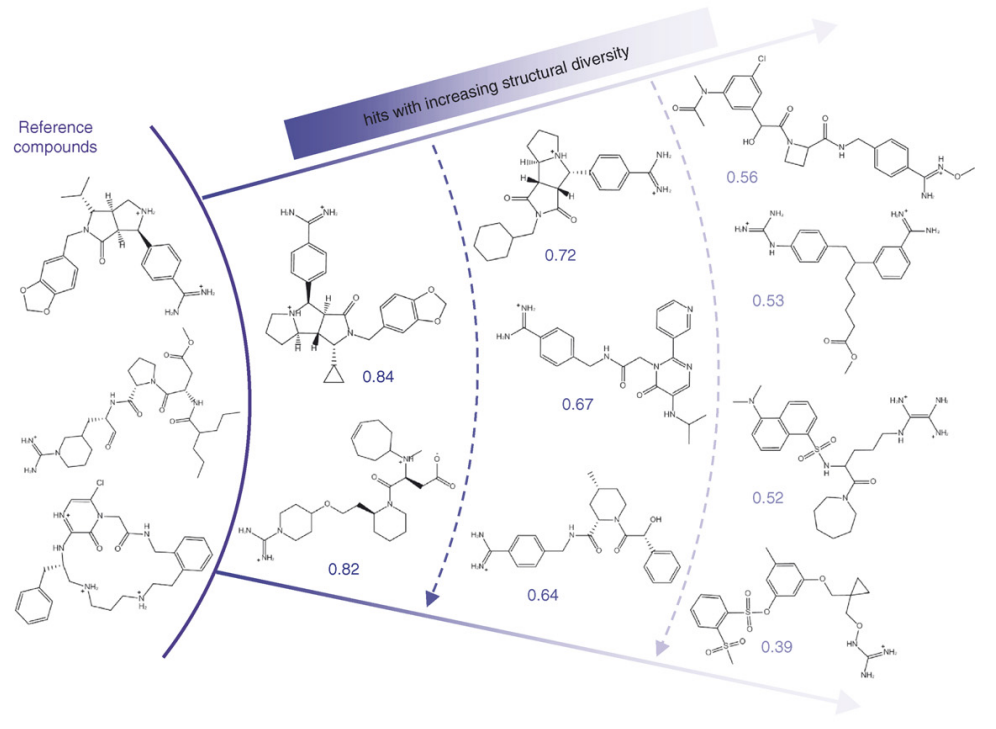
\includegraphics[scale=1.2]{Figuras/vs_diversity.png}
\caption{Espectro estrutural dos inibidores de trombina, onde o grau de similaridade foi obtido pelo coeficiente de Tanimoto. \cite{Eckert2007}}
\end{figure}

\section{Triagem baseada nas propriedades físico-químicas(ADME)}

Os atuais esforços de química medicinal estão produzindo compostos com maior massa molecular e $c \log P$ do que medicamentos de décadas atrás. Os fármacos mais recentes, desde 1990, possuem $c \log P$ mediano de 3,1 e massa molecular de 432 Da. Embora a preocupação com perfis farmacocinéticos sejam importantes, no desenvolvimento de medicamentos, a toxicidade também é crucial. O carácter lipofílico($\log P$) é a propriedade molecular mais importante a ser considerada para reduzir o risco de toxicidade. \cite{Leeson2007}

\section{O surgimento da Mecânica Quântica}

Por muito tempo, químicos e físicos acreditavam que as regras que governam os sistemas microscópicos e macroscópicos eram semelhantes. Então, em 1900, Max Planck ofereceu uma proposta radical de que a radiação emitida pelo corpo negra estava limitada a certos valores discretos, ou seja, estava ``quantizada". À medida que o século XX avançava, tornou-se cada vez mais claro que a quantização era não apenas uma característica da luz, mas também das partículas fundamentais das quais a matéria é constituída.  \cite{Cramer2004}

Há um limite intrínseco à precisão de nossa capacidade de observação e a pequenez da perturbação que o acompanha, um limite que é inerente à natureza das coisas e que talvez nunca possa ser superado por uma técnica aprimorada ou por uma habilidade maior por parte do observador. A causalidade se aplica apenas a sistemas que não sofrem perturbações relativamente significativas, e assim, surge uma mecânica cuja visão é probabilística. \cite{Dirac1958}

Para descrever sistemas microscópicos, então, uma mecânica diferente foi necessária.
Um candidato promissor foi a mecânica das ondas, já que ondas estacionárias também são quantizadas, como proposto inicialmente por De Broglie. No entanto, descobriu-se também apresentar propriedades semelhantes a partículas. Para explicar essa dicotomia, uma nova mecânica, a mecânica quântica, foi desenvolvida. \cite{Cramer2004}

O operador que retorna a energia do sistema, $E$, possui um valor próprio sendo denominado de
operador Hamiltoniano, $\hat{H}$. Tem-se então, a equação de \textit{Schr\"{o}dinger} para o átomo de hidrogênio. \cite{Cramer2004}

\begin{equation}
    \hat{H} \Psi(r, R) = E \Psi(r, R)
\end{equation}

A forma típica do operador Hamiltoniano leva em conta cinco contribuições para a energia total de um sistema:
as energias cinéticas dos elétrons e núcleos, a atração dos elétrons para os núcleos, e as repulsões intereletrônicas e internucleares. \cite{Cramer2004}

\begin{equation}
    H = - \sum_{i} \cfrac{\hbar^2}{2m_e} \nabla_i^2 - \sum_{k} \cfrac{\hbar^2}{2m_k} \nabla_k^2 - \sum_i\sum_k \cfrac{e^2 Z_k}{r_{ik}} + \sum_{i < j} \cfrac{e^2}{r_{ij}} + \sum_{k < l} \cfrac{e^2 Z_k Z_l}{r_{kl}}
\end{equation}

Em geral, há muitas autofunções $\Psi$ aceitáveis para uma dada molécula, cada uma
caracterizada por um autovalor associado $E$ distinto. Desta forma, existe um conjunto completo (talvez infinito) de $\Psi_i$ com autovalores $E_i$. Para facilitar uma manipulação futura, podemos assumir sem perda de generalidade de que essas funções de onda são ortonormais, isto é, para um sistema contendo uma única partícula, a função de onda depende de apenas três coordenadas: \cite{Cramer2004}

\begin{equation}
    \int \int \int \Psi_i \Psi_j dx dy dz = \delta_{ij}
\end{equation}

\begin{equation}
    \int \Psi_j H \Psi_i dr = E_i \delta_{ij}
\end{equation}

É importante destacar que a $Eq.(3.4)$ é crucial na determinação da energia molecular de um sistema. Todavia, a natureza real da função de onda e da solução exata da integral na $Eq.(3.4)$ é complexa e abstrata para uma analogia intuitiva. \cite{Cramer2004}

\subsection{O princípio variacional}

Será discutido os modelos físicos em sistemas moleculares de muitos corpos. Isto porque, funções de onda exatas para esses sistemas são extremamente difíceis de expressar porque os movimentos correlacionados de partículas possuem uma complexidade matemática muito alta. Sendo assim, para definir o estado fundamental de um sistema, podemos julgar a qualidade das funções de onda mediante suas energias associadas, de maneira a ser buscado o valor mínimo de energia do sistema ou estado de equilíbrio. \cite{Cramer2004}

Esse resultado é crítico porque nos mostra que não precisamos construir a suposta função de onda $\Psi$ como uma combinação linear de funções de onda ortonormais $\Psi_i$ (desconhecidas), mas podemos construí-la de várias maneiras distintas. \cite{Cramer2004}

\begin{equation}
    \Phi = \sum_i c_i \Psi_i
\end{equation}

\begin{equation}
    \int \Phi H \phi dr - E_0 \int \Phi^2 dr \geq 0
\end{equation}

\begin{equation}
     \cfrac{\mathlarger{\int} {\Phi H \Phi dr}}{\mathlarger{\int}{\Phi^2 dr}} \geq E_0
\end{equation}

A qualidade da aproximação será determinada pelo quão baixo for o valor calculado para a integral na $Eq. (3.7)$. Além disso, como precisamos encontrar as menores energia possíveis dentro das restrições de como construímos uma função de onda, pode-se usar todas as ferramentas que o Cálculo Diferencial e Integral disponibiliza para localizar valores extremos. \cite{Cramer2004}

\subsection{Aproximação de Born-Oppenheimer}



\subsection{Aproximação de Hartre-Fock}

\subsection{Teoria do Funcional da Densidade(DFT)}

\subsection{Funções de Base}

\subsection{Funcionais de Troca e Correlação}

\section{Docking Molecular}

Nos esforços da descoberta de medicamentos, é fundamental a compreensão dos mecanismos pelos quais os receptores de proteínas numa patologia reconhecem e interagem com os substratos moleculares ou inibidores. Apesar dos grandes avanços nos algoritmos de docking molecular nas últimas décadas, ainda existem muitas lacunas. Em particular, a ausência da flexibilidade de proteínas tem um aspecto crítico para uma melhor compreensão dos princípios que orientam a interações entre ligantes e proteínas. \cite{Souza2006}

A questão principal de todos os programas de docking é abordar qual combinação de orientação e conformação (pose) é a mais favorável em relação a todas as outras combinações possíveis(confôrmeros). Quando aplicado à triagem virtual, o processo também exige uma comparação da melhor conformação de um determinado ligante com a de outros possíveis ligantes, de modo que um pontuação(score) possa ser obtida. \cite{Perola2004}

Os softwares de docking molecular executam um algoritmo de busca no qual a conformação do ligante é avaliada recursivamente até que a convergência para a energia mínima seja alcançada. Finalmente, uma função de pontuação de afinidade, $\Delta G$ [U total em kcal / mol], é empregada para classificar as orientações mais favoráveis para a soma das energias eletrostática e van der Waals. \cite{Pagadala2017}

\begin{equation}
    N_{conf} = \prod^{N}_{i=1} \prod^{n_{inc}}_{j=1} \cfrac{360º}{\theta_{i, j}}
\end{equation}

Em uma busca conformacional sistemática, a $Eq.(3.8)$ fornece o número de possíveis conformações moleculares pelos seguintes parâmetros: $N$ é o número de ligações rotacionáveis e $\theta_{i, j}$ é o valor do incremento do ângulo de rotação $j$ da ligação $i$.\cite{Kitchen2004}

\subsection{Algoritmos de Busca}

Um rigoroso algoritmo de pesquisa elucidaria todos os modos de ligação possíveis entre o ligante e o receptor. Desta forma, consideraria todos os graus de translação e liberdade rotacional do ligante, como também os graus de liberdade conformacionais da proteína. No entanto, \cite{Taylor2002}

\subsection{Algoritmos Genéticos(GA) de busca}

Os genótipos são mapeados para fenótipos por uma função de mapeamento de desenvolvimento. Ao atingir iterações suficientes da pesquisa local a ponto de encontrar o mínimo local, uma função de mapeamento inverso é usada para converter seu fenótipo em seu genótipo correspondente. No docking molecular, a pesquisa local é realizada pela conversão contínua do genótipo para o fenótipo.

O estado do ligante corresponde ao genótipo, enquanto suas coordenadas atômicas correspondem ao fenótipo. No encaixe molecular, a afinidade é a energia total de interação do ligante com a proteína. O cromossomo é composto de uma sequência de genes de valor real: três coordenadas cartesianas para a tradução do ligante; quatro variáveis que definem um quatérnion especificando a orientação do ligante; e um valor real para cada torção do ligante, respectivamente. 

No desenvolvimento do AutoDock Vina, diversas abordagens estocásticas de otimização global foram exploradas, incluindo algoritmos genéticos. No algoritmo, há uma sucessão de etapas que consistem em uma mutação e uma otimização local, sendo cada etapa aceita de acordo com o critério de Metropolis. Durante a implementação, foi adotado o método Broyden-Fletcher-Goldfarb-Shanno(BFGS) para a otimização local, que é um eficiente método quasi-Newton. \cite{Vina2010}

\begin{figure}[H]
\centering
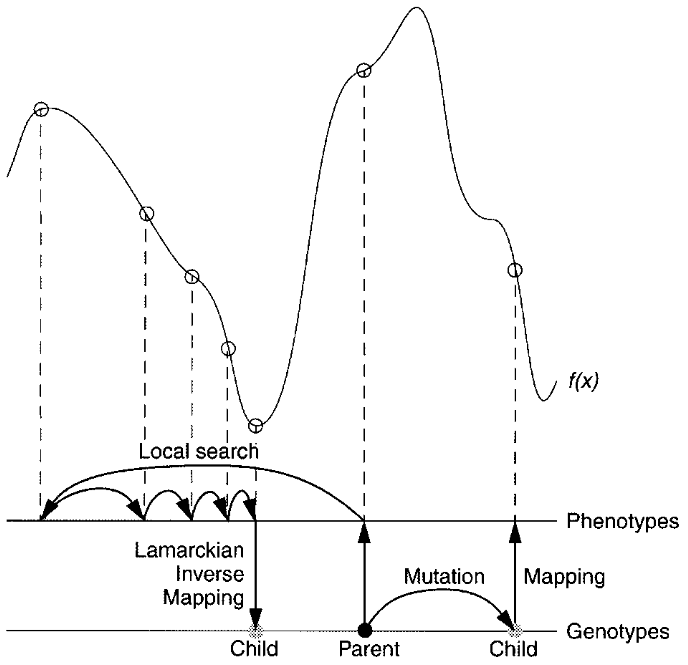
\includegraphics[scale=1.35]{Figuras/lga_search.png}
\caption{É ilustrado o algoritmo de busca Lamarckiano(LGA), assim como a busca de um mínimo local mediante a conversão e mutação recursiva entre genótipos e o respectivo fenótipo. \cite{Autodock1998}}
\end{figure}

\subsection{Algoritmos de Scoring}

Num campo de força AMBER utilizado nos softwares AutoDock(1998) e AutoDock Vina(2010), para dois átomos $i, j$, a energia atômica em pares é avaliada pela soma das interações de van der Waals, ligações de hidrogênio, energia de Coulomb e dessolvatação. \cite{Autodock1998} A função de score do AutoDock 4 foi calibrada a partir de 30 dados experimentais de proteínas em complexo. A implementação tem como base o ciclo termodinâmico de Wesson-Eisenberg.\cite{Autodock1998} No AutoDock Vina, a função de score é uma combinação de abordagem empírica, devido à calibração por meio de 1300 complexos proteicos, e baseada no conhecimento físico-químico das interações proteína-ligante. \cite{Vina2010}

\begin{equation}
    \Delta G_{obs} = RT \ln {K_i}
\end{equation}

A calibração da função de scoring foi a partir de valores experimentais de $\Delta G$, onde $K_i$ representa a constante de inibição. \cite{Autodock1998}

\begin{equation}
    \Delta G_{binding} = \Delta G_{vdW} + \Delta G_{elec} + \Delta G_{hbond} + \Delta G_{desolv} + \Delta G_{tors}
\end{equation}

$\Delta G_{vdW} \rightarrow$ Representa o potencial de Lennard-Jones para dispersão e repulsão intereletrônica; \\

$\Delta G_{elec} \rightarrow$ Efeitos eletrostáticos baseados no modelo dielétrico de Solmajer \& Mehler; \\

$\Delta G_{hbond} \rightarrow$ Potencial das ligações de hidrogênio conforme o modelo da direcionalidade de Goodford's; \\

$\Delta G_{desolv} \rightarrow$ Dessolvatação por meio do emparelhamento de Stouten; \\

$\Delta G_{desolv} \rightarrow$ Energia livre associada às ligações rotacionáveis. \\

A $Eq. (3.11)$ representa o modelo físico utilizado pelo AutoDock4 como função para estimar a energia livre total entre receptor-ligante: \cite{Autodock1998}

\begin{equation}
\begin{split}
       V = W_{vdw} \sum_{i,j} \left( \cfrac{A_{ij}}{r_{ij}^{12}} - \cfrac{B_{ij}}{r_{ij}^6} \right) + W_{hbond} \sum_{i,j} E(t) \left(  \cfrac{C_{ij}}{r_{ij}^{12}} - \cfrac{D_{ij}}{r_{ij}^{10}}    \right) + W_{elec} \sum_{i,j} \cfrac{q_i q_j}{\epsilon(r_{ij}) r_{ij}} + \\ W_{sol} \sum_{i, j} (S_i V_j + S_j V_i) e^{(-r_{ij}^2/2\sigma^2)}
\end{split}
\end{equation}

\section{Avaliação dos resultados de docking}

Existem dois modos de RMSD: O RMSD absoluto e o RMSD relativo. O RMSD absoluto mede a distância entre pares de átomos correspondentes sem translação ou rotação de coordenadas. Entretanto, o RMSD relativo implica uma etapa de alinhamento(simetrização) adicional do moléculas antes do cálculo RMSD real. \cite{Kirchmair2008}

\begin{equation}
    <RMSD_{lb}(c1, c2)> = max(rmsd'(c1, c2), rmsd'(c2, c1))
\end{equation}

\begin{equation}
    <RMSD'_{ab}> = \sqrt{\cfrac{1}{N} \sum_{i} min_{j} r_{ij}^2}
\end{equation}

A precisão das \textit{poses} de encaixe é quantificada pelo cálculo do RMSD entre o valor experimental da estrutura ligante determinada e a calculada pelo algoritmo de busca. Atualmente, o RMSD entre uma pose de encaixe gerada e a conformação experimental do ligante representa a referência mais estabelecida para o sucesso do algoritmo de predição da conformação. \cite{Kirchmair2008} O valor de corte RMSD de $2 \si{\angstrom}$  é frequentemente usado como critério da validade de predição do docking proteína-ligante. \cite{Bursulaya2003} 

\section{Teorias de interação proteína-ligante}

A teoria \textit{``chave-fechadura''} proposta por \textit{Fisher} em 1894, considerava o receptor rígido e imóvel ancorando em um ligante sem sofrer quaisquer rearranjos conformacionais(conformação reativa). Em contrapartida, foi largamente abandonada em favor de modelos de ligação que não apenas consideram alterações conformacionais, mas também um ajuste estocástico de receptores e ligantes. \cite{Durrant2011} Desta forma, o encaixe induzido(em termos modernos, desestabilização do estado fundamental) advém da teoria do estado de transição, a hipótese de complementaridade enzima-ligante. \cite{Benkovic2003}

\begin{figure}[H]
\centering
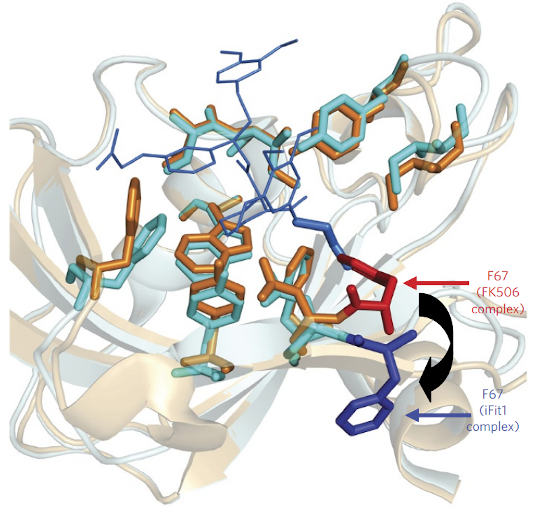
\includegraphics[scale=0.35]{Figuras/induced_fit2.png}
\caption{Inibidores da proteína FKBP51 interagem pelo mecanismo de encaixe induzido, causando mudanças conformacionais no complexo receptor-ligante.  \cite{Gaali2015}}
\end{figure}

\section{Limitações dos algoritmos de docking}

A maior limitação dos métodos de docking é o modelo rígido do receptor. O AutoDock e o AutoDock Vina permitem flexibilidade limitada das cadeias laterais do receptor. Para sistemas com movimentos maiores de loops ou domínios, uma variedade de conformações do receptor pode ser calculada mediante dinâmica molecular e, em seguida, realizam-se simulações de docking a partir de snapshots. \cite{Autodock2016}

A água desempenha um papel crítico na termodinâmica da interação receptor-ligante. A contabilização exata dos efeitos da solvatação/dessolvatação ainda permanece um desafio significativo. \cite{Yuriev2015}

